\chapter{Teoretické východiská}

\section{Arduino}
Arduino je open-source platforma používaná na vytváranie elektronických projektov. Samotná platforma pozostáva z fyzickej, programovateľnej vývojovej dosky pripojiteľnej typicky cez USB a vývojového prostredia pre počítače~\cite{maly-hvj}.

Pod názvom Arduino bolo vytvorených množstvo verzií vývojových dosiek, v našej práci sa zameriame na verziu Arduino Uno (Rev3).

\subsection{Arduino Uno}
Jadrom dosky Arduino Uno je mikrokontrolér ATmega328P pracujúci na frekvencii 16 MHz. Samotná doska obsahuje 14 digitálnych (z toho 6 PWM) a 6 analógových vývodov. Taktiež obsahujuje 32 kB flash pamäte, 2 kB pamäte SRAM a 1 kB pamäte EEPROM~\cite{arduino-uno}.

\begin{figure}
    \centering
    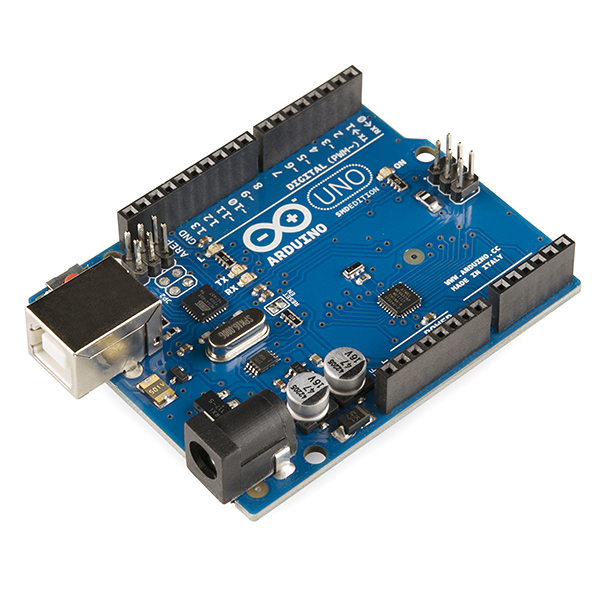
\includegraphics{img/Arduino_Uno.jpg}
    \caption{Arduino Uno.}
\end{figure}

\subsection{Vývojové prostredie}
Pre vývoj programov je primárne určené vývojové prostredie Arduino IDE. Podporuje vývoj v jazykoch C a C++ a obsahuje štandardnú knižnicu z projektu Wiring~\cite{maly-hvj}.

\begin{figure}
    \centering
    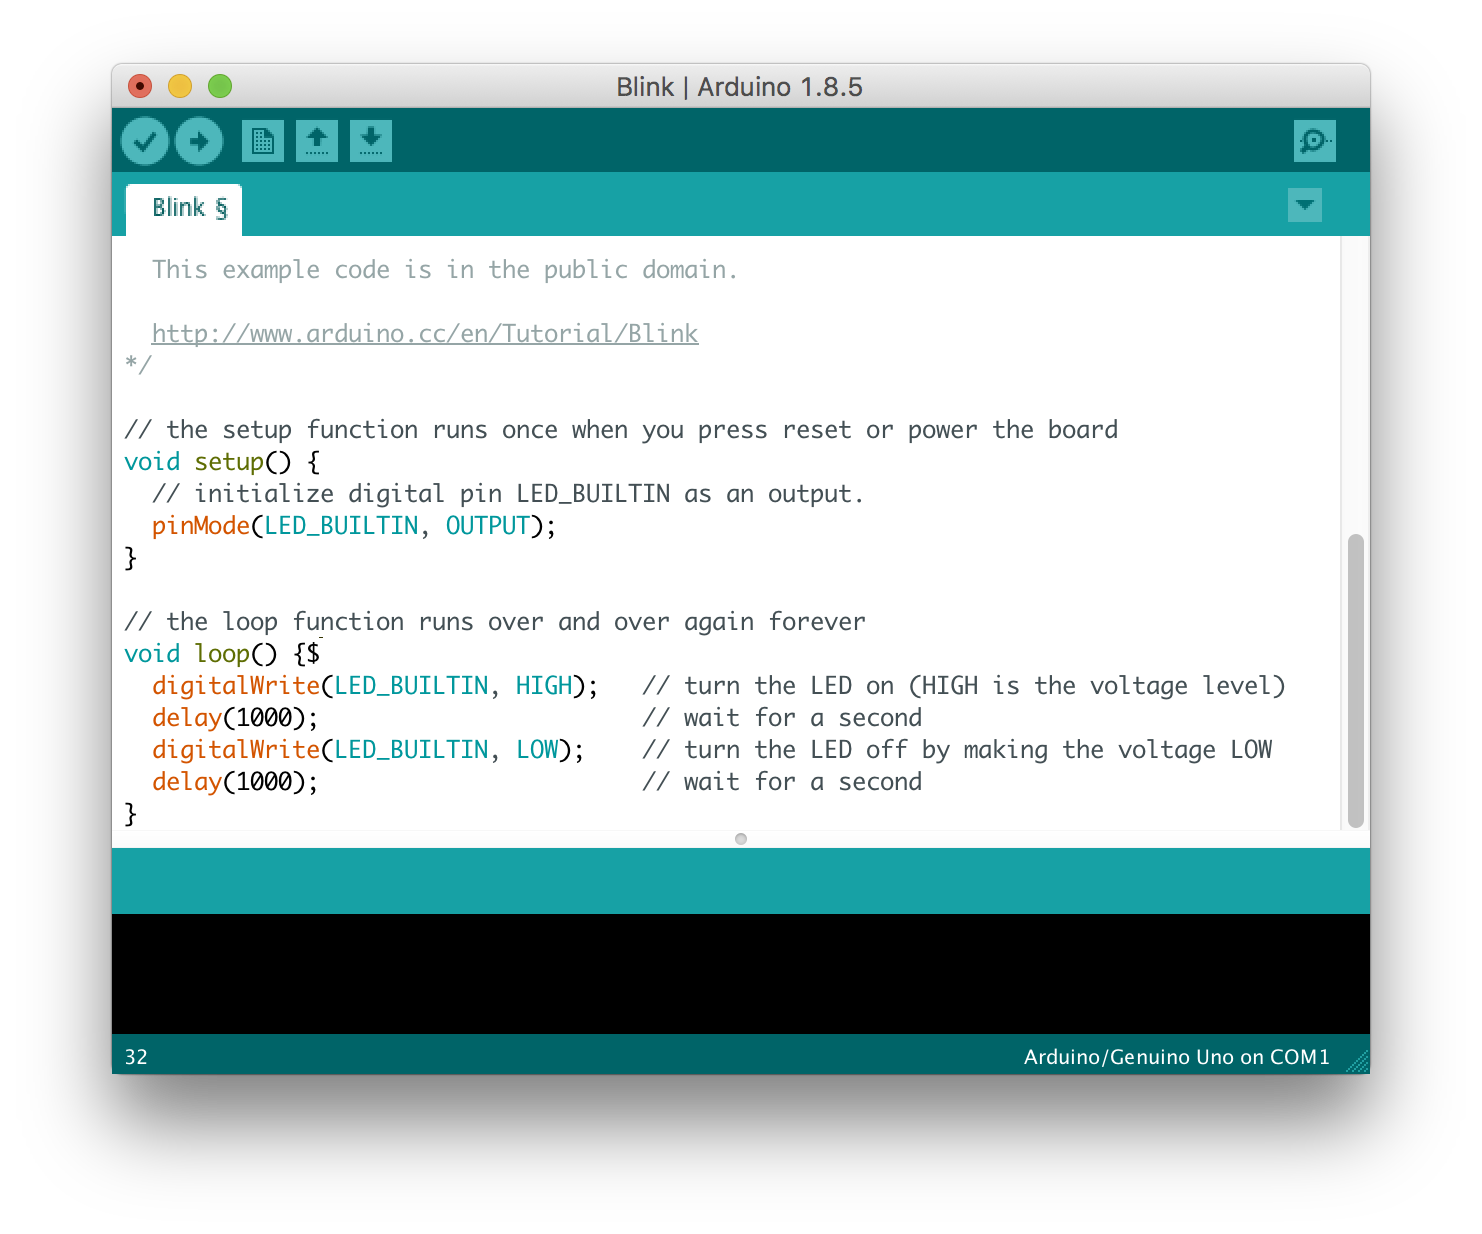
\includegraphics[width=\textwidth]{img/Arduino_IDE.png}
    \caption{Vývojové prostredie Arduino IDE.}
\end{figure}

Programovanie pre Arduino má niektoré odlišnosti oproti bežnému programovaniu v C/C++. Samotný program sa v Arduino terminológií nazýva \emph{sketch} a musí obsahovať 2 funkcie: jednu pre inicializáciu (\texttt{void setup()}) a druhá obsahuje hlavný cyklus programu (\texttt{void loop()})~\cite{maly-hvj}.

\section{Modul reálneho času}
Nakoľko pre budík je udržovanie presného údaju o aktuálnom čase kriticky dôležité, je vhodné využiť pre tento účel modul reálneho času (RTC). Jedná sa o integrovaný obvod ktorý sleduje skutočný čas nezávisle od ostatných súčastí systému~\cite{rtc-adafruit}. Vďaka zálohovacej batérií funguje aj pri strate hlavného napájania.

Hardvér samotného Arduina RTC neobsahuje, je však možné ho jednoducho pripojiť.
%\section{LCD Display}
